\documentclass[./main.tex]{subfiles}

\begin{document}

\subsection{Product perspective}

The following diagram formally describes the relations between the
entities taken into account in the description of the world and of the
shared phenomena. More specifically, it provides a clear point of view
on which types of users can access the developed services, and shows how
SafeStreets interfaces with external resources to exploit back-end
processes.

\begin{figure}[H]
\centering
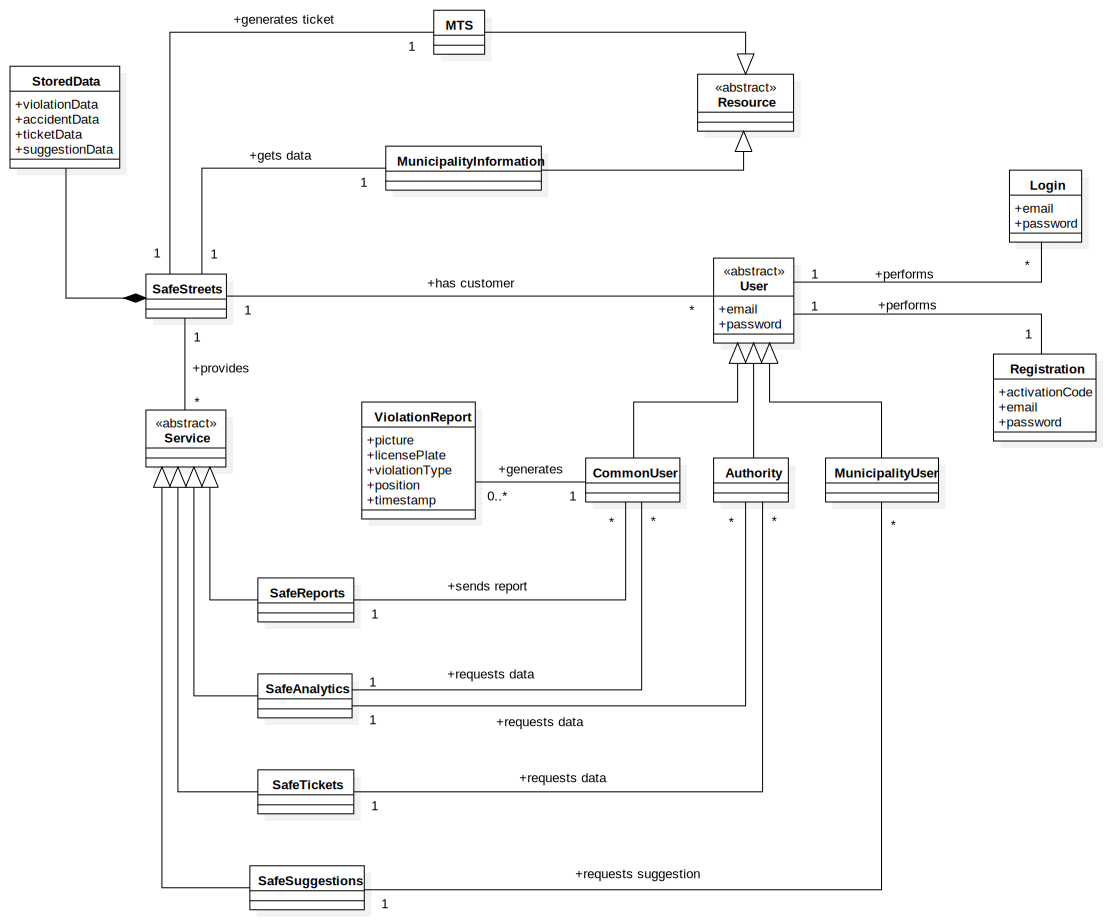
\includegraphics[width=\textwidth]{class_diagram}
\caption{Class diagram}
\end{figure}

As mentioned in the previous section, a service is exploited differently
depending on the type of user that is enjoying it. This is important
when considering SafeAnalytics, which has a crucial role in the
application, but is developed both to common users and authorities.
These types of users have different rights when accessing data stored by
SafeStreets, and will be provided with different query interfaces to
make their requests. If referring to the diagram, one could think to the
classes as the processes inherent to specific functionalities, and to
the relations as the interfaces provided to the users to enjoy a
service.\\
Relations between application and the resources do not need further
explanation, as they are deeply analyzed in the following sections to
describe how the interaction works.

\subsubsection{State diagrams}

In the diagrams shown below are emphasized the possible states of the
entities, and the transitions between one state to another.

\begin{figure}[H]
\centering
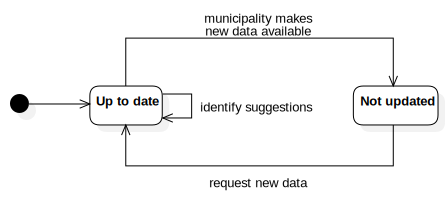
\includegraphics[width=\textwidth]{state_diagram_application}
\caption{Application}
\end{figure}

\begin{figure}[H]
\centering
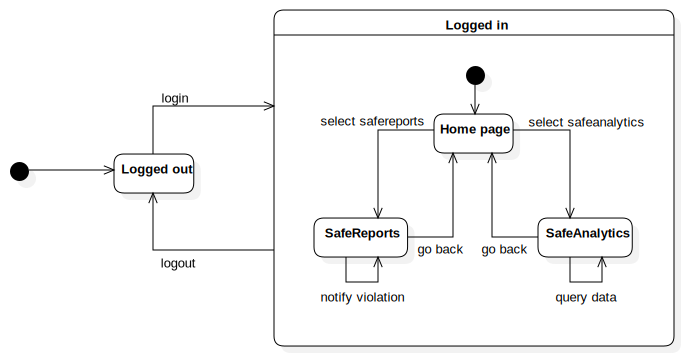
\includegraphics[width=\textwidth]{state_diagram_common_user}
\caption{Common user}
\end{figure}

\begin{figure}[H]
\centering
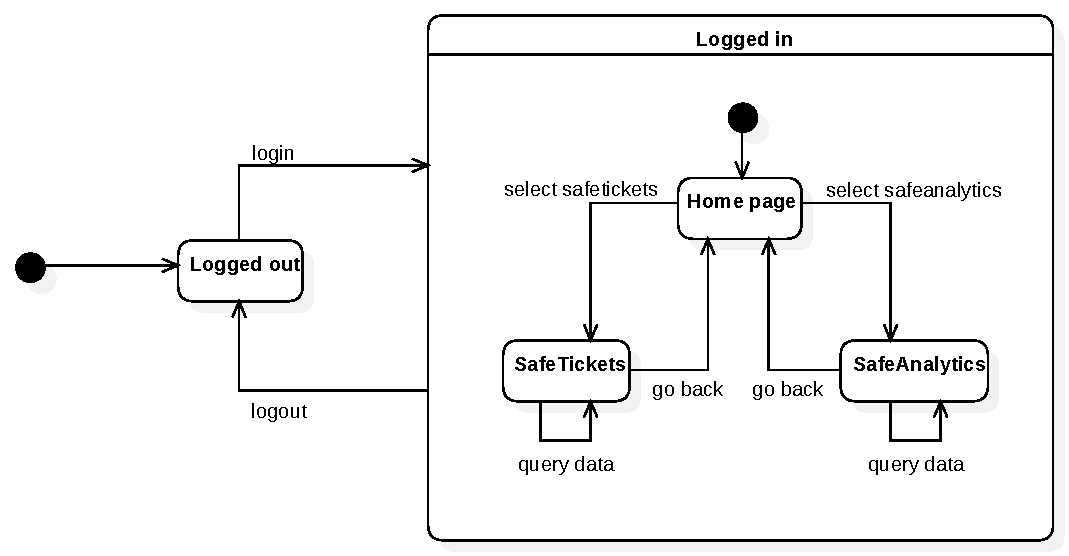
\includegraphics[width=\textwidth]{state_diagram_authority}
\caption{Authority}
\end{figure}

\begin{figure}[H]
\centering
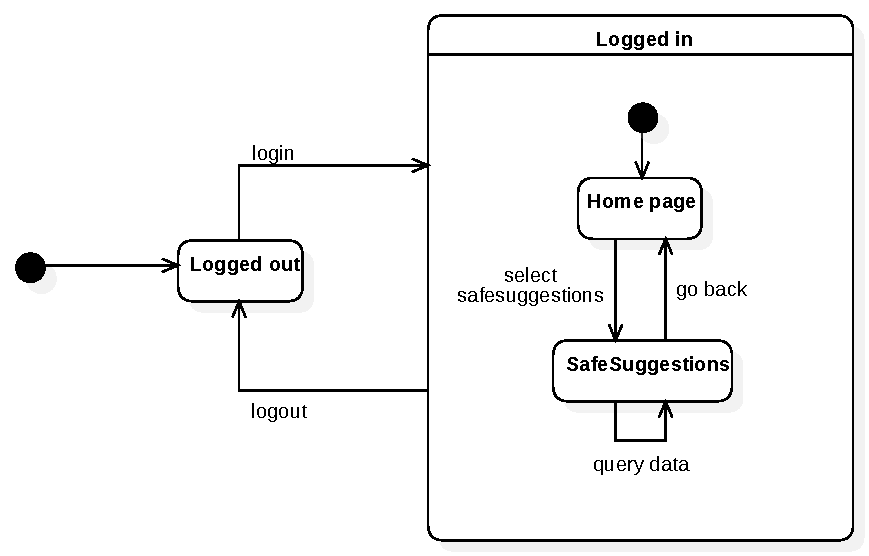
\includegraphics[width=\textwidth]{state_diagram_municipality_user}
\caption{Municipality user}
\end{figure}

\subsection{Product functions}

This section focuses on the definition of the functions to be provided
to reach the goals previously listed. For each service, a set of
requirements is identified. Later on in the document, these requirements
will be revised and factored to be mapped on the goals.

\subsubsection{SafeReports}

\begin{itemize}
\item
  The service must allow users to take pictures.
\item
  The service must forward pictures to OCR software to detect license
  plates.
\item
  The service must detect the timestamp.
\item
  The service must detect the position of the user.
\item
  The service must create a violation report filling it with the needed
  data.
\item
  The service must ask confirmation to the user before sending the
  violation report.
\item
  The service must check the integrity of the violation report before
  storing it.
\item
  The service must check for duplicated events before storing the
  violation report.
\item
  The service must forward stored violation report to MTS.
\item
  The service must store information on issued tickets when forwarding
  violation reports.
\end{itemize}

\subsubsection{SafeAnalytics}

\begin{itemize}
\item
  The service must provide users with a query interface.
\item
  The service must allow common users to select a time interval in the
  query interface.
\item
  The service must allow common users to select a day as a minimum
  granularity of the time interval.
\item
  The service must allow common users to select a zone in the query
  interface.
\item
  The service must allow common users to select 1 kilometer as the
  minimum granularity of the zone.
\item
  The service must allow common users to select a violation type in the
  query interface.
\item
  The service must allow authorities to access a special query
  interface.
\item
  The service must allow authorities to consult all the information
  stored.
\item
  The service must allow authorities to select a license plate in the
  special query interface.
\item
  The service must allow authorities to see the pictures of the
  violations.
\item
  The service must allow authorities to filter data using any
  granularity.
\end{itemize}

\subsubsection{SafeTickets}

\begin{itemize}
\item
  The service must provide authorities with a query interface.
\item
  The service must allow authorities to consult all the stored data
  about issued tickets.
\item
  The service must allow authorities to use the same filters of
  SafeAnalytics.
\item
  The service must allow going back to the violation report from which
  the tickets were generated.
\end{itemize}

\subsubsection{SafeSuggestions}

\begin{itemize}
\item
  The service must provide municipality users with a query interface.
\item
  The service must allow municipality users to request a suggestion
  using the query interface.
\item
  The service must allow municipality users to select a type of
  violation in the query interface.
\item
  The service must allow municipality users to select a zone in the
  query interface.
\item
  The service must provide suggestions to reduce the incidence of the
  selected violation in the selected zone.
\end{itemize}

\subsection{User characteristics}

As previously mentioned, several types of users can be identified. Every
type of user has different needs and limitations, that must be satisfied
providing different services. In this section, users are analyzed with
relation to their characteristics, to formally define these needs and
limitations.

\subsubsection{Common users}

Common users are the core of the application and the channel through
which the application collects data. Common users contribute to building
the data set that they can query to get data about violations. They must
be guided through the process of notification to make it easy and
intuitive and must be provided with the possibility to select the
correct filters to query the stored data.

\subsubsection{Authorities}

Authorities are, from a certain point of view, supervisors of the stored
data. They are not provided with the possibility to notify violations
(it is not what the authority account was designed for), but they can
access all the stored data about both notified violations and issued
tickets. For this type of account is not so important the easiness of
the interaction. Instead, it is very important to provide authorities
with the possibility to use powerful filters to query data.

\subsubsection{Municipality users}

The needs of the municipality users are somehow disjoint from those of
other users. This type of account is designed to give the possibility to
get the suggestions identified by the application. Because of this,
municipality users are not provided with the possibility to query the
stored data or to notify violations. Instead, they are provided with a
special query interface that allows them to select filters depending on
which type of intervention they want to put in place.

\subsection{Assumptions and dependencies}

\subsubsection{Domain assumptions}

\begin{itemize}
\item
  \textbf{D1} Users do not modify reality to generate fake violation
  reports.
\item
  \textbf{D2} The violations notified by the users are coherent with the
  taken pictures.
\item
  \textbf{D3} There exists a finite set of violations.
\item
  \textbf{D4} There exists a finite number of possible interventions.
\item
  \textbf{D5} Devices running SafeStreets has a working camera.
\item
  \textbf{D6} The camera is always safe (it is not possible to alter the
  data acquired by the camera).
\item
  \textbf{D7} Devices running SafeStreets are always able to get the
  timestamp.
\item
  \textbf{D8} Devices running SafeStreets are always able to detect the
  position with an error of at least 5 meters.
\item
  \textbf{D9} Internet connection is supposed to work whenever a user
  wants to use SafeStreets.
\item
  \textbf{D10} If OCR software returns a result, it is supposed to be
  correct.
\item
  \textbf{D11} If OCR software is not able to recognize a plate, it
  returns a special response.
\item
  \textbf{D12} A violation report is anonymous if and only if it
  consists only of the type of violation, position, and date.
\item
  \textbf{D13} Authorities and municipality users are previously
  verified.
\item
  \textbf{D14} Data from the municipality is reliable.
\end{itemize}

\subsubsection{Dependencies}

There are not strong dependencies between the services developed by the
application. There is a clear distinction between services that store
data and services that access data, thanks to this they can be exploited
independently one from each other. It is obvious that accessing the same
data set, it is useless to exploit services without storing data, so the
utility of the query services is bound to the existence of data
collection services.

\begin{itemize}
\item
  SafeAnalytics is based on data collection through SafeReports.
\item
  SafeTickets is based on the data collection from MTS.
\item
  SafeSuggestions is based on the data collection from the municipality
  data set.
\end{itemize}

Stronger dependencies exist between SafeStreets and the external
services to whom some tasks are delegated.

\begin{itemize}
\item
  SafeReports uses external OCR software.
\item
  SafeStreets is based on the GoogleMaps API.
\end{itemize}

The characteristic of these dependencies is that the link is not
exclusive with the service to which the tasks are delegated, in the
sense that services can be changed. OCR software can be any, and
OpenStreetMaps API can be used instead of GoogleMaps ones.

\end{document}